\begin{frame}{4D flow MRI in one slide}
\small
\begin{columns}[T]
\begin{column}{0.55\textwidth}
\begin{itemize}
\item Measure blood velocity $v(r,\tau)\in\RR^3$ over the cardiac cycle with a \emph{phase} contrast: the MR signal phase depends on velocity (explained next).
\item Data: Fourier-like samples, 32 coils, 10 minutes. Target: 1\,mm resolution, whole thorax.
\item Per frame and encode we have $\sim2\%$ of the samples of a fully sampled image.
\end{itemize}
\end{column}
\begin{column}{0.45\textwidth}
\centering
\begin{tikzpicture}[node distance=4mm,every node/.style={draw,rounded corners,align=center,font=\scriptsize,minimum width=2.6cm}]
\node (a) {physics $\Phi(r,t)$\\\textbf{Part 1}};
\node[below=of a] (b) {velocity encoding $E$\\\textbf{Part 2}};
\node[below=of b] (c) {reconstruction $x_{k+1}=D(\cdot)$\\\textbf{Part 3}};
\node[below=of c] (d) {symmetric denoiser $D$\\\textbf{Part 4}};
\draw[->] (a)--(b); \draw[->] (b)--(c); \draw[->] (c)--(d);
\end{tikzpicture}
\end{column}
\end{columns}
\medskip
Four mathematical problems, each easy to state, each (partly) open. No solutions in this talk, only the questions.
\end{frame}

\begin{frame}{What 4D flow data look like (simulated phantom)}
\centering
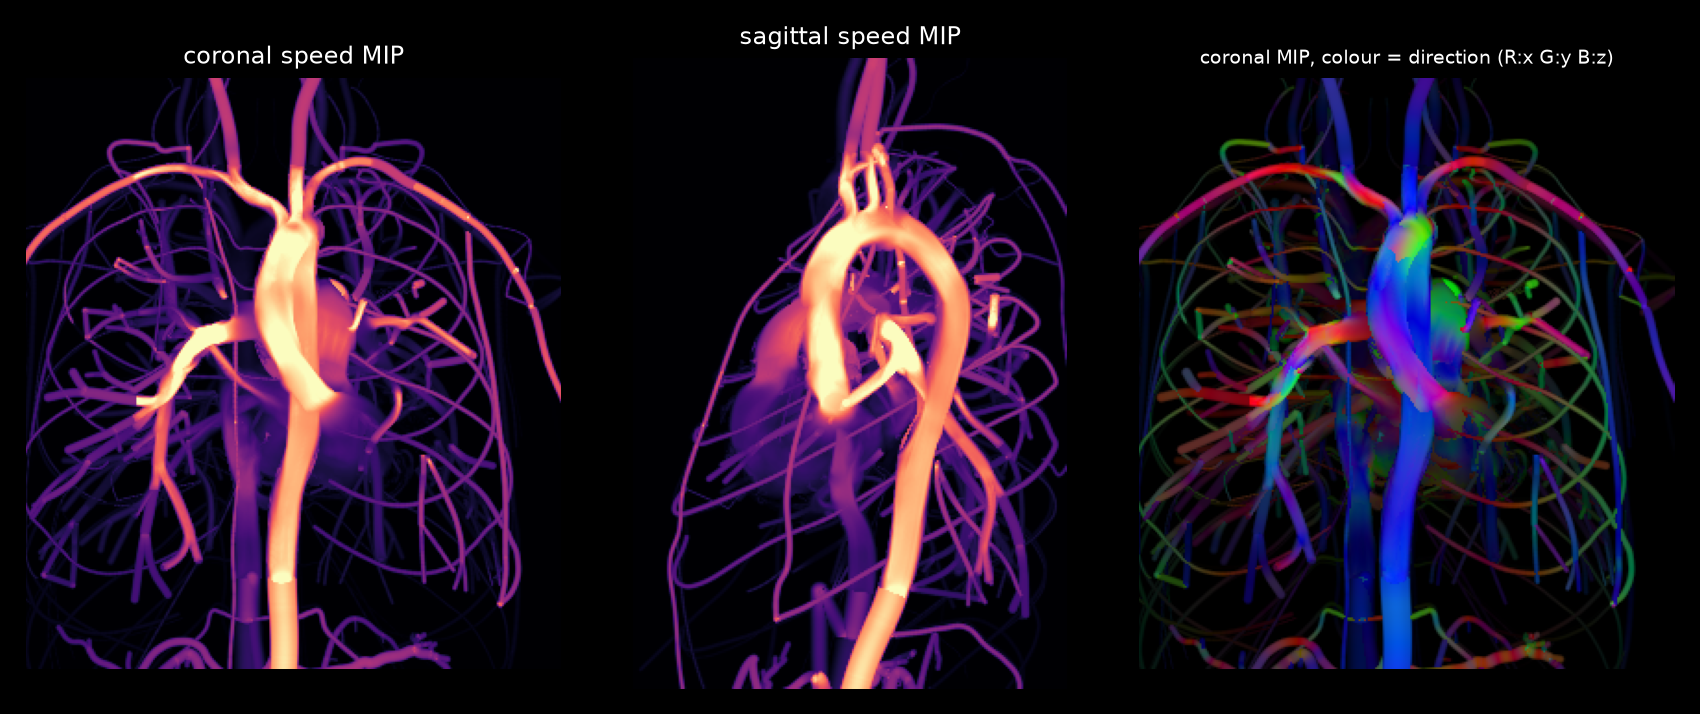
\includegraphics[width=0.93\textwidth]{figs/flow_mip.png}\\[1mm]
{\footnotesize Peak-systole blood-speed maximum-intensity projections (MIPs) of a CFD-driven simulated subject at 1\,mm; right panel colours the direction of flow. The scanner measures such a volume at $\sim$20 time frames per heartbeat. (Simulation, not scanner data.)}
\end{frame}

\iflong
\begin{frame}{The simulated subject: vessel network}
\centering
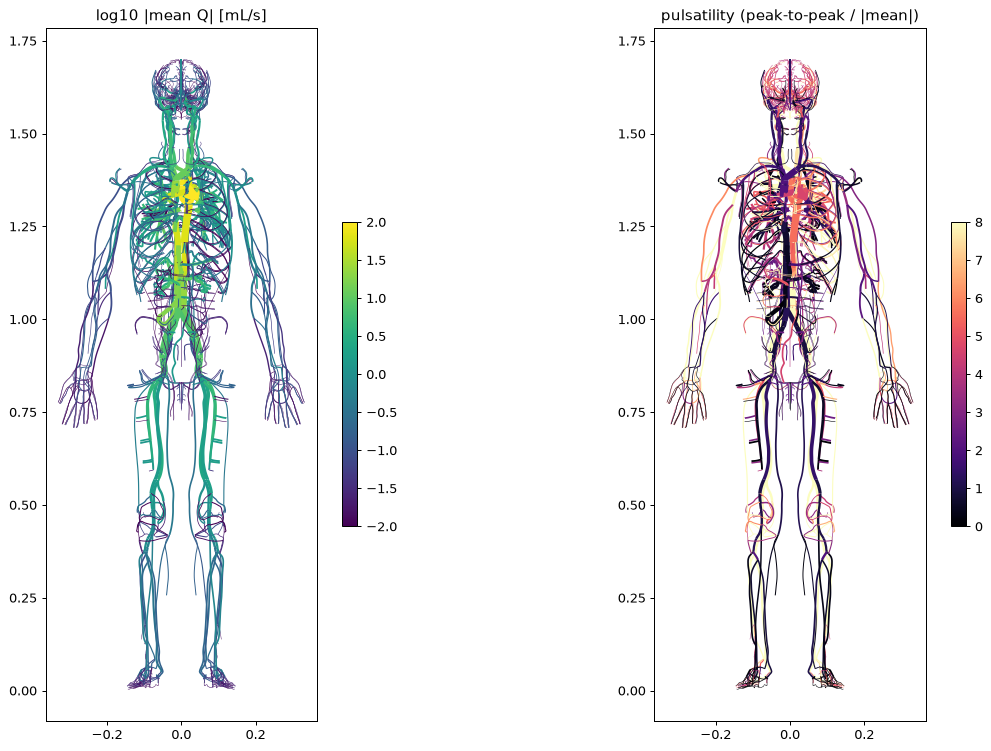
\includegraphics[height=0.72\textheight]{figs/vessel_network.png}\\[1mm]
{\footnotesize Whole-body vessel network of the simulated subject: mean flow (left, log scale) and pulsatility (right).}
\end{frame}
\begin{frame}{The simulated subject: heart chamber flow}
\centering
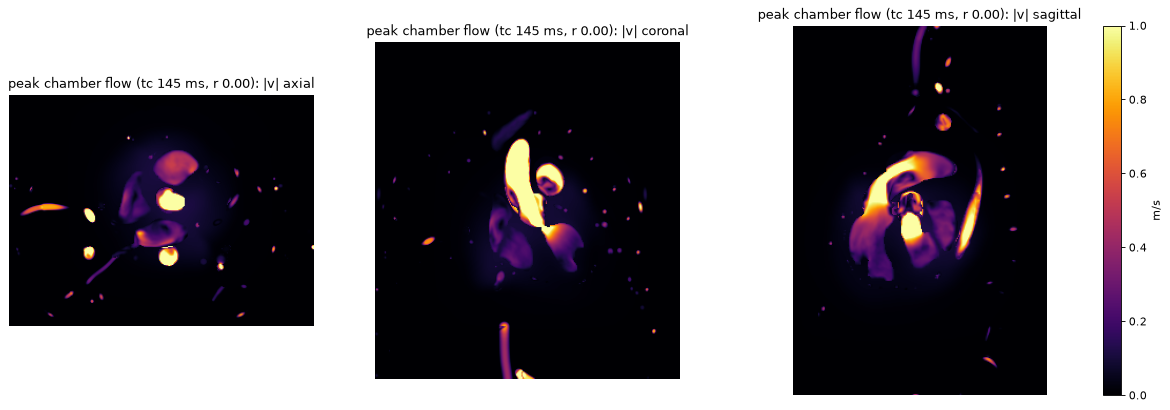
\includegraphics[width=0.92\textwidth]{figs/chamber_flow.png}\\[1mm]
{\footnotesize Blood speed at peak chamber flow (axial, coronal, sagittal slices) from lattice-Boltzmann CFD of the heart.}
\end{frame}
\fi
